\documentclass{article}
\usepackage{tikz}

\begin{document}

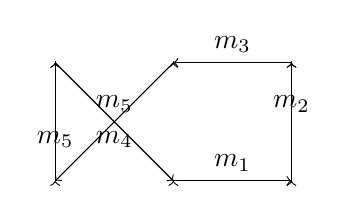
\begin{tikzpicture}[scale=1.5]
    % Define coordinates for the vertices
    \coordinate (A) at (0,0);
    \coordinate (B) at (1,0);
    \coordinate (C) at (1,1);
    \coordinate (D) at (0,1);
    \coordinate (E) at (-1,0);
    \coordinate (F) at (-1,1);

    % Draw the edges with arrows
    \draw[->] (A) -- node[above] {$m_1$} (B);
    \draw[->] (B) -- node[above] {$m_2$} (C);
    \draw[->] (C) -- node[above] {$m_3$} (D);
    \draw[->] (D) -- node[below] {$m_4$} (E);
    \draw[->] (E) -- node[below] {$m_5$} (F);
    \draw[->] (F) -- node[above] {$m_5$} (A);

    % Draw the loops
    \draw[->] (A) to [out=90,in=90] (A);
    \draw[->] (B) to [out=-90,in=-90] (B);
    \draw[->] (C) to [out=180,in=180] (C);
    \draw[->] (D) to [out=0,in=0] (D);
    \draw[->] (E) to [out=90,in=90] (E);
    \draw[->] (F) to [out=-90,in=-90] (F);
\end{tikzpicture}

\end{document}